\scanpage{35}
% archive sheet number: 34
{\unsure{Difficulté|Difficile}}

\diagram{\begin{tikzcd}[ampersand replacement=\&,column sep=large,row sep=large]
0\arrow[r]\&\underset{\substack{\text{faisceau de}\\\text{Picard relatif}\\\text{\uline{{\unsure{réduit}}} (?)}}}{\underline{{\unsure{\mathscr{P}|\Phi}}}(X/Y)_0}\arrow[r]\&\underline{\operatorname{Ext}}^1(\mathscr{P}^0_{X/Y},G_m)\arrow[d,"{\unsure{2|\sim}}","\substack{\text{\uline{autodualité de}}\\\text{\uline{la Jacobienne}}}"']\\
\&\&\deleted{{\unsure{\mathscr{P}^0}}}\underline{H}^0(Y,\mathscr{P}^0_{X/Y})
\end{tikzcd}}
\figure{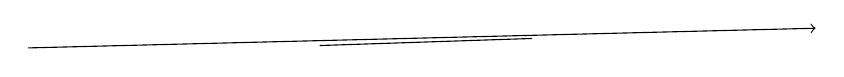
\begin{tikzpicture}\draw[->] (0,0)--(10,.25);\draw (3.7,.03)--(6.4,.12);\end{tikzpicture}}
\margin{sur ${\unsure{Y}}$}
La réciproque semble {\unsure{vraie}} pour les faisceaux de {\unsure{Weil}}. Ceci dit, on doit avoir sous des conditions convenables
\diagram{\begin{tikzcd}[ampersand replacement=\&,column sep=large,row sep=small]
\underline{\underline{H}}^*(X_S/{\unsure{Y}},G)\&\underline{\underline{\operatorname{Ext}}}^*(\mathscr{P}_S,G)\arrow[l,"\sim"']\arrow[d,"2"]\\
\&\underline{\underline{\operatorname{Ext}}}^{{\unsure{2|*|\geq}}}(\mathscr{P}_S^0,G)\quad\text{en }\underline{\underline{\text{dim }>0}}
\end{tikzcd}}
D'autre part, on a \deleted{{\unsure{une}}} \inserted{des} suites spectrales,
\[
\begin{aligned}
\operatorname{Ext}^*(\mathscr{P}_S,G)&\Longleftarrow H^p(Y,\underline{\underline{\operatorname{Ext}}}^{q}(\mathscr{P}_S,G))\\
\underset{\deleted{\underline{\phantom{H}}}}{H}^*(X_S/Y,G)&\Longleftarrow H^p({\unsure{Y}},\underline{\underline{H}}^q(X_S/Y,G))
\end{aligned}
\]
d'où en \deleted{substituant une suite spectrale}
\[
\deleted{\boxed{H^*(X_S/Y,G)\Longleftarrow H^p(Y,\underline{\underline{\operatorname{Ext}}}^{q}(\mathscr{P}_S,G))}}
\]
\deleted{d'où une suite exacte à 5 termes}

{\unsure{comprenant}} le résultat plausible
\[
{\unsure{H}}^*(X_S/Y,G)\simeq\operatorname{Ext}_S^*(\mathscr{P}_S,G)
\]
\margin{$\deleted{0\longrightarrow H^1(Y,\underline{\operatorname{Hom}}(\mathscr{P}_S,G))}$}
